%%%%%%%%%%%%%%%%%%%%%%%%%%%%%%%%%%%%%%%%%%%%%%%%%%%%%%%%%%%%%%%%%%%%%%%%%%%%%%%%
%2345678901234567890123456789012345678901234567890123456789012345678901234567890
%        1         2         3         4         5         6         7         8
% DOCUMENT CLASS
\documentclass[oneside,12pt]{Classes/RoboticsLaTeX}

% USEFUL PACKAGES
% Commonly-used packages are included by default.
% Refer to section "Book - Useful packages" in the class file "Classes/RoboticsLaTeX.cls" for the complete list.
\usepackage{amsmath}
\usepackage{amsfonts}
\usepackage{algorithm}
\usepackage{algorithmic}

% SPECIAL COMMANDS
% correct bad hyphenation
\hyphenation{op-tical net-works semi-conduc-tor}
%% ignore slightly overfull and underfull boxes
%\hbadness=10000
%\hfuzz=50pt
% declare commonly used operators
\DeclareMathOperator*{\argmax}{argmax}

% HEADER
\ifpdf
    \pdfinfo {/Title (Example of PhD Thesis with RoboticsLaTeX template)
              /Creator (TeX)
              /Producer (pdfTeX)
              /Author (Barbara Bruno, Fulvio Mastrogiovanni)
              /CreationDate (D:20141024182500) %format D:YYYYMMDDhhmmss
              /ModDate (20141024182500)
              /Subject (Example of PhD Thesis with RoboticsLaTeX template)
              /Keywords (PhD, Thesis, Example, RoboticsLaTeX)}
    \pdfcatalog {/PageMode (/UseOutlines)
                 /OpenAction (fitbh) }
\fi

\title{Example of PhD Thesis with RoboticsLaTeX template}

\ifpdf
  \author{\href{mailto:barbara.bruno@unige.it}{Barbara Bruno}
          \href{mailto:fulvio.mastrogiovanni@unige.it}{Fulvio Mastrogiovanni}}
  \collegeordept{\href{http://www.dibris.unige.it}{DIBRIS - Department of Computer Science, Bioengineering, Robotics and System Engineering}}
  \university{\href{http://www.unige.it}{University of Genova}}
  \crest{
\includegraphics[width=30mm]{logo_unige}}
\else
  \author{Barbara Bruno, Fulvio Mastrogiovanni}
  \collegeordept{DIBRIS - Department of Computer Science, Bioengineering, Robotics and System Engineering}
  \university{University of Genova}
  \crest{
\includegraphics[width=30mm]{logo_unige}}
\fi

% DECLARATION
% Use the following command to change the declaration text:
%\renewcommand{\submittedtext}{INSERT NEW TEXT HERE}
\degree{Doctor of Philosophy}
\degreedate{February 31, 2015}

%%%%%%%%%%%%%%%%%%%%%%%%%%%%%%%%%%%%%%%%%%%%%%%%%%%%%%%%%%%%%%%%%%%%%%%%%%%%%%%%

\begin{document}

% A page with the abstract and running title and author etc may be
% required to be handed in separately. If this is not so, comment
% the following 3 lines:
% \begin{abstractseparate}
%   %%%%%%%%%%%%%%%%%%%%%%%%%%%%%%%%%%%%%%%%%%%%%%%%%%%%%%%%%%%%%%%%%%%%%%%%%%%%%%%%
%2345678901234567890123456789012345678901234567890123456789012345678901234567890
%        1         2         3         4         5         6         7         8
% THESIS ABSTRACT

% Use the following style if the abstract is long:
%\begin{abstractslong}
%\end{abstractslong}

\begin{abstracts}

This is a very short and uninformative abstract.

\end{abstracts}

% \end{abstractseparate}

\maketitle

% add an empty page after title page
\newpage\null\thispagestyle{empty}\newpage

% set the number of sectioning levels that get number and appear in the contents
\setcounter{secnumdepth}{3}
\setcounter{tocdepth}{3}

\frontmatter
%%%%%%%%%%%%%%%%%%%%%%%%%%%%%%%%%%%%%%%%%%%%%%%%%%%%%%%%%%%%%%%%%%%%%%%%%%%%%%%%
%2345678901234567890123456789012345678901234567890123456789012345678901234567890
%        1         2         3         4         5         6         7         8
% THESIS ACKNOWLEDGEMENTS

% Use the following style if the acknowledgements are long:
%\begin{acknowledgementslong}
%\end{acknowledgmentslong}

\begin{acknowledgements}


Don't forget to acknowledge your supervisor!


\end{acknowledgements}

%%%%%%%%%%%%%%%%%%%%%%%%%%%%%%%%%%%%%%%%%%%%%%%%%%%%%%%%%%%%%%%%%%%%%%%%%%%%%%%%
%2345678901234567890123456789012345678901234567890123456789012345678901234567890
%        1         2         3         4         5         6         7         8
% THESIS DEDICATION

\begin{dedication}

To all the Master and PhD students of Robotics Engineering at the University of Genova.
\end{dedication}

% ----------------------------------------------------------------------

%%% Local Variables: 
%%% mode: latex
%%% TeX-master: "../thesis"
%%% End: 

%%%%%%%%%%%%%%%%%%%%%%%%%%%%%%%%%%%%%%%%%%%%%%%%%%%%%%%%%%%%%%%%%%%%%%%%%%%%%%%%
%2345678901234567890123456789012345678901234567890123456789012345678901234567890
%        1         2         3         4         5         6         7         8
% THESIS ABSTRACT

% Use the following style if the abstract is long:
%\begin{abstractslong}
%\end{abstractslong}

\begin{abstracts}

This is a very short and uninformative abstract.

\end{abstracts}


\tableofcontents
\listoffigures
%\printglossary  % Print the nomenclature (WAY TOO COMPLEX FOR ME NOW!)
%\addcontentsline{toc}{chapter}{Nomenclature}

\mainmatter
%%%%%%%%%%%%%%%%%%%%%%%%%%%%%%%%%%%%%%%%%%%%%%%%%%%%%%%%%%%%%%%%%%%%%%%%%%%%%%%%
%2345678901234567890123456789012345678901234567890123456789012345678901234567890
%        1         2         3         4         5         6         7         8
% THESIS INTRODUCTION

\chapter{Introduction}
\label{chap:introduction}
\ifpdf
    \graphicspath{{Introduction/Figures/PNG/}{Introduction/Figures/PDF/}{Introduction/Figures/}}
\else
    \graphicspath{{Introduction/Figures/EPS/}{Introduction/Figures/}}
\fi

Write the Introduction here...

%%%%%%%%%%%%%%%%%%%%%%%%%%%%%%%%%%%%%%%%%%%%%%%%%%%%%%%%%%%%%%%%%%%%%%%%%%%%%%%%
%2345678901234567890123456789012345678901234567890123456789012345678901234567890
%        1         2         3         4         5         6         7         8
% THESIS CHAPTER

\chapter{First chapter}
\label{chap:first}
\ifpdf
    \graphicspath{{Chapter1/Figures/PNG/}{Chapter1/Figures/PDF/}{Chapter1/Figures/}}
\else
    \graphicspath{{Chapter1/Figures/EPS/}{Chapter1/Figures/}}
\fi

% short summary of the chapter
\section*{Summary}

Examples of commonly used commands.

\section{Basic commands}
\label{sec:basic_commands}

This is a citation: \cite{Cox91}.

This is an emphasized word: \emph{global}.

This is a reference to another part of the thesis: Chapter \ref{chap:introduction}.

This is an enumerated list:
\begin{enumerate}
\item first item.
\item second item.
\end{enumerate}

This is an in-line equation: $x-$.

This is a word in quotes: ``regular''.

\section{Equation}
\label{sec:equation}

This is an equation:
\begin{equation}
{\mathcal{U}}_k(s_k) = \frac{P_k}{C_k}
\label{eq:normal}
\end{equation}

This is an equation split over multiple lines:
\begin{equation}
\begin{array}{l}
x_{k}={\mathcal{F}}(x_{k-1},u_{k},w_{k-1})\\
z_{k}={\mathcal{H}}(x_{k},v_{k})
\label{eq:Split}
\end{array}
\end{equation}

This is one hell of an equation:
\begin{equation}
\begin{array}{c}
 \mathcal{Q}_l  = \frac{{d_l ^2 \sigma _\phi  ^2 }}{2}\left[ {\begin{array}{cc}
   {2\sin ^2 \phi _l } & { - \sin 2\phi _l }  \\
   { - \sin 2\phi _l } & {2\cos ^2 \phi _l }  \\
\end{array}} \right] +
 \begin{array}{cc}
   {\frac{{\sigma _d ^2 }}{2}\left[ {\begin{array}{cc}
   {2\cos ^2 \phi _l } & {\sin 2\phi _l }  \\
   {\sin 2\phi _l } & {2\sin ^2 \phi _l }  \\
\end{array}} \right]}  \\
\end{array} \\
 \end{array}
\label{eq:defQ}
\end{equation}

This is a reference to the Equation \ref{eq:Split}.

\section{Figure}
\label{sec:figure}

I add a figure.
\begin{figure}
\centering
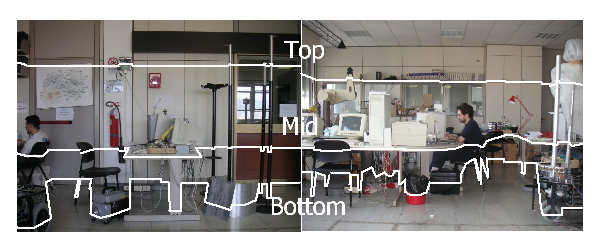
\includegraphics[width=5.0in]{Views}
\caption{Scan profiles: \emph{bottom}, \emph{mid} and \emph{top view}.}
\label{fig:views}
\end{figure}

This is a reference to Figure \ref{fig:views}.

\section{Algorithm} 
\label{sec:algorithm}

This is an algorithm:
\begin{algorithm}
\label{alg:SMS}
\caption{Split \& Merge [\& Split]}
\begin{algorithmic} [1]
\REQUIRE{A scan $s$. A stack $\mathcal{L}$. A counter $j$. A threshold $\tau$}
\ENSURE{$\lambda \leftarrow \mathcal{M}(s)$, $j=1, ..., |\lambda|$}
\STATE{$\mathcal{L}$ = \texttt{push}($s$)}
\STATE{$j \leftarrow 1$}
\WHILE{$\mathcal{L}$ $\neq$ $\varnothing$}
\STATE{$\mathcal{L}$ = \texttt{pop}($s_{top}$)}
\STATE{$l_j$ $\leftarrow$ \texttt{fitting}($s_{top}$)}
\STATE{$q_k = \argmax_{q}\texttt{dist(l$_j$,q)}$}
\IF{$\texttt{dist(l$_j$,$q_k$)} < \tau$}
\STATE{$j \leftarrow j+1$}
\STATE{\texttt{continue}}
\ELSE
\STATE{$s_a \leftarrow$ \texttt{sub}($s_{top}$, 1, $k$)}
\STATE{$s_b \leftarrow$ \texttt{sub}($s_{top}$, $k+1$, $|s|$)}
\STATE{$\mathcal{L}$ = \texttt{push}($s_a$)}
\STATE{$\mathcal{L}$ = \texttt{push}($s_b$)}
\ENDIF
\ENDWHILE
\STATE{\{$l_j$\} $\leftarrow$ \texttt{merge}(\{$l_j$\})}
\STATE{\{$l_j$\} $\leftarrow$ \texttt{split}(\{$l_j$\})}
\end{algorithmic}
\end{algorithm}
%%%%%%%%%%%%%%%%%%%%%%%%%%%%%%%%%%%%%%%%%%%%%%%%%%%%%%%%%%%%%%%%%%%%%%%%%%%%%%%%
%2345678901234567890123456789012345678901234567890123456789012345678901234567890
%        1         2         3         4         5         6         7         8
% THESIS CONCLUSIONS
\def\baselinestretch{1}
\chapter{Conclusions}
\label{chap:conclusions}
\ifpdf
    \graphicspath{{Conclusions/Figures/PNG/}{Conclusions/Figures/PDF/}{Conclusions/Figures/}}
\else
    \graphicspath{{Conclusions/Figures/EPS/}{Conclusions/Figures/}}
\fi
\def\baselinestretch{1.66}

Write the conclusions here...

\appendix
%%%%%%%%%%%%%%%%%%%%%%%%%%%%%%%%%%%%%%%%%%%%%%%%%%%%%%%%%%%%%%%%%%%%%%%%%%%%%%%%
%2345678901234567890123456789012345678901234567890123456789012345678901234567890
%        1         2         3         4         5         6         7         8
% THESIS APPENDIX

\chapter{Extra}
\label{chap:appendixA}

Write here...

\bibliographystyle{Classes/RoboticsBiblio}    % bibliography style
\renewcommand{\bibname}{References}           % change default name Bibliography to References
\bibliography{References/references}          % References file
\addcontentsline{toc}{chapter}{References}    % add References to contents page

\end{document}
